\chapter{Spin 1/2 Field}
\section{Representation of the Lorentz group}
Recall that
\[U^{-1}(\Lambda) \phi_a(x) U(\Lambda) = \mathscr{S}_{a}^{\phantom{a}b}\phi_b(\Lambda^{-1}x).\]
For infinitesimal rotation,
\[\mathscr{S}_{a}^{\phantom{a}b} = \delta_{a}^{\phantom{a}b}+\frac{i}{2} \delta \omega_{\alpha \beta} (\mathcal{S}^{\alpha \beta})_{a}^{\phantom{a}b} .\]
Matrices $\mathcal{S}^{\alpha \beta}$ satisfy the following commutation relation
\[[\mathcal{S}^{\mu \nu},\mathcal{S}^{\rho \sigma}]= -\eta^{\nu \rho}\mathcal{S}^{\mu \sigma} + \eta^{\sigma \mu}\mathcal{S}^{\rho \nu} + \eta^{\mu \rho}\mathcal{S}^{\nu \sigma} - \eta^{\sigma \nu}\mathcal{S}^{\rho \mu}.\]
Define $\mathcal{C}_i \equiv \frac{1}{2}\epsilon_{ijk}\mathcal{S}^{jk}$,$\mathcal{D}_i \equiv \mathcal{S}^{i0}$, we have
\[[\mathcal{C}_i,\mathcal{C}_j] = i\epsilon_{ijk}\mathcal{C}_k , \quad [\mathcal{C}_i,\mathcal{D}_j] = i\epsilon_{ijk}\mathcal{D}_k , \quad [\mathcal{D}_i,\mathcal{D}_j] = -i\epsilon_{ijk}\mathcal{C}_k.\]
We further define $\mathcal{N}_i \equiv \frac{1}{2}(\mathcal{C}_i-i\mathcal{D}_i)$ and $\mathcal{N}^{\dagger}_i \equiv \frac{1}{2}(\mathcal{C}_i + i \mathcal{D}_i)$, then the commutation relation will be
\[[\mathcal{N}_i,\mathcal{N}_j] = i\epsilon_{ijk}\mathcal{N}_k , \quad [\mathcal{N}^{\dagger}_i,\mathcal{N}^{\dagger}_j] = i\epsilon_{ijk}\mathcal{N}^{\dagger}_k , \quad [\mathcal{N}_i,\mathcal{N}^{\dagger}_j] = 0.\]
We see that we have two different $\mathrm{SU}(2)$ Lie algebras that are exchanged by hermitian conjugation. As we just discussed, a representation of the $\mathrm{SU}(2)$ Lie algebra is specified by an integer or half integer; we therefore conclude that a representation of the Lie algebra of the Lorentz group in four spacetime dimensions is specified by two integers or half-integers $n$ and $n'$.
\\ \\
We will label these representations as $(2n+1, 2n'+1)$; the number of components of a representation is then $(2n+1)(2n'+1)$. Different components within a representation can also be labelled by their angular momentum representations. We have $\mathcal{C}_i = \mathcal{N}_i + \mathcal{N}^{\dagger}_i$. Thus, deducing the allowed values of $j$ given $n$ and $n'$ becomes a standard problem in the addition of angular momenta. The general result is that the allowed values of $j$ are $|n-n'|,|n-n'|+1,\cdots, n+n'$, and each of these values appears exactly once.

\section{Spin--statistics theorem}
\begin{newthem}[Spin--statistics theorem]
States with identical particles of integer spin are symmetric under the interchange of the particles, while states with identical particles of half-integer spin are antisymmetric under the interchange of the particles.
This is equivalent to the statement that the creation and annihilation operators for integer spin particles satisfy canonical commutation relations, while creation and annihilation operators for half-integer spin particles satisfy canonical anti-commutation relations.
Particles quantized with canonical commutation relations are called bosons, and satisfy Bose--Einstein statistics, and particles quantized with canonical anti-commutation relations are called fermions, and satisfy Fermi--Dirac statistics.
\end{newthem}

\noindent
Roughly speaking,  one way to interchange two particles is to rotate them around their midpoint by $\pi$. For a particle of spin $s$, this rotation will introduce a phase factor of $e^{i\pi s}$. Thus, a two-particle state with identical particles both of spin $s$ will pick up a factor of $e^{i2\pi s}$. For $s$ a half-integer, this will give a factor of $-1$; for $s$ an integer, it will give a factor of $+1$. Therefore, the creation and annihilation operators for integer spin particles satisfy canonical commutation relations, while creation and annihilation operators for half-integer spin particles satisfy canonical anti-commutation relations. The detailed proof can be found in chapter 12.1 and 12.2 from \emph{Quantum Field Theory and the Standard Model (Matthew D. Schwartz)}.

\section{Spinor field}
Consider a left-handed spinor field $\psi_a(x)$, also known as a left-handed Weyl field, which is in the $(2,1)$ representation of the Lie algebra of the Lorentz group. Here the index $a$ is a left-handed spinor index that takes on two possible values. Under a Lorentz transformation, we have
\[U(\Lambda)^{-1} \psi_a(x) U(\Lambda) = L_a^{\phantom{a}b}(\Lambda) \psi_b(\Lambda^{-1}x).\]
For an infinitesimal transformation, we can write
\[L_a^{\phantom{a}b}(1+\delta \omega) = \delta_a^{\phantom{a}b} + \frac{i}{2} \delta \omega_{\mu \nu} (\mathcal{S}_{\rm L}^{\mu \nu})_a^{\phantom{a}b}.\]
$n=1,\, n'=0$  implies that
\[(\mathcal{S}_{\rm L}^{i j}) = \frac{1}{2}\epsilon^{ijk}\sigma_k , \quad  (\mathcal{S}_{\rm L}^{k 0}) = \frac{1}{2}i\sigma_k,\]
where $\sigma_k$ is Pauli matrix.
Then the infinitesimal transformation can be written as
\[L(1+\delta \omega) = I - \frac{i}{2} \theta_i \sigma_i -\frac{1}{2} \beta_i \sigma_i.\]
Recall that hermitian conjugation swaps the two $\mathrm{SU}(2)$ Lie algebras that comprise the Lie algebra of the Lorentz group.
Therefore, the hermitian conjugate of a field in the $(2,1)$ representation should be a field in the $(1,2)$ representation; such a field is called a right-handed spinor field or a right-handed Weyl field. We will distinguish the indices of the $(1,2)$ representation from those of the $(2,1)$ representation by putting dots over them. Thus, we write
\[[\psi_a(x)]^{\dagger} = \psi^{\dagger}_{\dot{a}}(x).\]
Under a Lorentz transformation, we have
\[U(\Lambda)^{-1} \psi^{\dagger}_{\dot{a}}(x) U(\Lambda) = R_{\dot{a}}^{\phantom{a}\dot{b}}(\Lambda) \psi^{\dagger}_{\dot{b}}(x)(\Lambda^{-1}x).\]
For an infinitesimal transformation, we can write
\[R_{\dot{a}}^{\phantom{a}\dot{b}}(1+\delta \omega) = \delta_{\dot{a}}^{\phantom{a}\dot{b}} + \frac{i}{2} \delta \omega_{\mu \nu} (\mathcal{S}_{\rm R}^{\mu \nu})_{\dot{a}}^{\phantom{a}\dot{b}}.\]
We can prove that
\[(\mathcal{S}_{\rm R}^{\mu \nu})_{\dot{a}}^{\phantom{a}\dot{b}} = -[(\mathcal{S}_{\rm L}^{\mu \nu})_a^{\phantom{a}b}]^*.\]

\noindent
Define
\[\epsilon_{ab} \equiv \left[ \begin{matrix} 0& -1\\ 1& 0\end{matrix} \right] .\]
Group theory can show that
\[L_a^{\phantom{a}c}(\Lambda) L_b^{\phantom{b}d}(\Lambda) \epsilon_{cd} = \epsilon_{ab},\]
which means that $\epsilon_{ab}$ is an invariant symbol of the Lorentz group: it does not change under a Lorentz transformation that acts on all of its indices. The inverse matrix of $\epsilon_{ab}$ is
\[\epsilon^{ab} \equiv \left[ \begin{matrix} 0& 1\\ -1& 0\end{matrix} \right] .\]
Thus
\[\epsilon_{ab}\epsilon^{bc} = \delta_a^{\phantom{a}c} , \quad \epsilon^{ab}\epsilon_{bc} = \delta^a_{\phantom{a}c}.\]
We can use $\epsilon_{ab}$ and and its inverse $\epsilon^{ab}$ to raise and lower left-handed spinor indices, 
\[\psi^a(x) \equiv \epsilon^{ab} \psi_b(x).\]
We also notice the minus sign when we contract indices,
\[\psi^a \chi_a = -\psi_a \chi^a.\]
We can verify the following equations:
\[-L^a_{\phantom{a}b} L_a^{\phantom{a}c} = \delta^c_b .\]
\[\psi_a(x) = \epsilon_{ab} \psi^b(x).\]
\[L^a_{\phantom{a}c}(\Lambda) L^b_{\phantom{b}d}(\Lambda) \epsilon^{cd} = \epsilon
^{ab}.\]
\[U(\Lambda)^{-1} \psi^a(x) U(\Lambda) = -L^a_{\phantom{a}b}(\Lambda) \psi^b(\Lambda^{-1}x).\]
In right handed representation, we can also deduce the existence of an invariant symbol $\epsilon_{\dot{a}\dot{b}}$. The value of $\epsilon_{\dot{a}\dot{b}}$ is the same as that of $\epsilon_{ab}$.
Define
\[\sigma^{\mu}_{a\dot{a}} \equiv (I,\vec{\sigma}).\]
It is an invariant symbol of the group $(2,1) \otimes (1,2) \otimes (2,2)$.
The properties of invariance symbol can be used to derive the following equations. The detailed derivation can be found in chapter 35 from \emph{Quantum Field Theory (Mark Srednicki)}.

\begin{newprop}
\begin{enumerate}
\item 
\[\sigma^{\mu}_{a\dot{a}} \sigma_{\mu b\dot{b}} = -2\epsilon_{ab} \epsilon_{\dot{a}\dot{b}}.\]
\[\epsilon^{ab}\epsilon^{\dot{a}\dot{b}} \sigma^{\mu}_{a\dot{a}} \sigma^{\nu}_{b\dot{b}} = -2\eta^{\mu\nu}.\]
\item \[(\mathcal{S}_{\rm L}^{\mu\nu})_{ab} = (\mathcal{S}_{\rm L}^{\mu\nu})_{ba}.\]
\[(\mathcal{S}_{\rm R}^{\mu\nu})_{\dot{a}\dot{b}} = (\mathcal{S}_{\rm R}^{\mu\nu})_{\dot{b}\dot{a}}.\]
\item Define
\[\overline{\sigma}^{\mu \dot{a} a} \equiv \epsilon^{ab} \epsilon^{\dot{a}\dot{b}} \sigma^{\mu}_{b\dot{b}}.\]
Numerically,
\[\overline{\sigma}^{\mu \dot{a} a} = (I , -\vec{\sigma}).\]
Thus
\begin{eqnarray}
(\mathcal{S}_{\rm L}^{\mu\nu})_a^{\phantom{a}b} &=& + \frac{i}{4} (\sigma^{\mu} \overline{\sigma}^{\nu} - \sigma^{\nu} \overline{\sigma}^{\mu})_a^{\phantom{a}b}, \nonumber \\
(\mathcal{S}_{\rm R}^{\mu\nu})^{\dot{a}}_{\phantom{\dot{a}} \dot{b}} &=& - \frac{i}{4}(\overline{\sigma}^{\mu}\sigma^{\nu} - \overline{\sigma}^{\nu} \sigma^{\mu})^{\dot{a}}_{\phantom{\dot{a}} \dot{b}}. \nonumber
\end{eqnarray}
\end{enumerate}
\end{newprop}

\noindent
We adopt the following convention: a missing pair of contracted,
undotted indices is understood to be written as $\phantom{1}^c_{\phantom{c}c}$, and a missing pair of
contracted, dotted indices is understood to be written as $\phantom{1}_{\dot{c}}^{\phantom{c}\dot{c}}$. Thus, if $\chi$ and
$\psi$ are two left-handed Weyl fields, we have
\[\chi \psi = \chi^{a}\psi_{a} , \quad \chi^{\dagger} \psi_{\dagger} = \chi^{\dagger}_{\dot{a}} \psi^{\dagger \dot{a}}.\]
We expect Weyl fields to describe spin-one-half particles, and (by the spin--statistics theorem) these particles must be fermions. Therefore the corresponding fields must anticommute, rather than commute. That is, we should have
\[\chi_a(x) \psi_b(y) = - \psi_b(x) \chi_a(x).\]
Thus, we can get
\[\chi\psi = \psi\chi.\]
Using the above convention, we can derive the following proposition:

\begin{newprop}
\begin{enumerate}
\item \[(\chi\psi)^{\dagger} = \psi^{\dagger}\chi^{\dagger}.\]
\item \[[\psi^{\dagger} \overline{\sigma}^{\mu} \chi]^{\dagger} = \chi^{\dagger} \overline{\sigma}^{\mu} \psi.\]
\end{enumerate}
\end{newprop}

\section{Lagrangians for spinor fields}
\subsubsection{Weyl field}
\[\mathcal{L} = i \psi^{\dagger} \overline{\sigma}^{\mu} \partial_{\mu} \psi .\]
\begin{note}
\[(i \psi^{\dagger} \overline{\sigma}^{\mu} \partial_{\mu} \psi)^{\dagger} = i \psi^{\dagger} \overline{\sigma}^{\mu} \partial_{\mu} \psi - \partial_{\mu}(i \psi^{\dagger} \overline{\sigma}^{\mu} \psi).\]
The second term is a total divergence, and vanishes (with suitable boundary conditions on the fields at infinity) when we integrate it over $d^4 x$ to get the action $S$. Thus $i \psi^{\dagger} \overline{\sigma}^{\mu} \partial_{\mu} \psi$  has the hermiticity properties necessary for a term in $\mathcal{L}$.
\end{note}
\noindent
We can derive the equation of motion from Hamilton principle,
\[\overline{\sigma}^{\mu} \partial_{\mu} \psi = 0.\]

\subsubsection{Majorana field}
If we add mass terms to the Lagrangian, we have
\[\mathcal{L} = i \psi^{\dagger} \overline{\sigma}^{\mu} \partial_{\mu} \psi - \frac{1}{2}m \psi \psi - \frac{1}{2}m \psi^{\dagger} \psi^{\dagger}.\]
The equation of motion is
\[-i\overline{\sigma}^{\mu} \partial_{\mu} \psi + m \psi^{\dagger} = 0 , \quad -i\sigma^{\mu} \partial_{\mu} \psi^{\dagger} + m \psi = 0 .\]
Define gamma matrix as
\[\gamma^{\mu} \equiv \left[ \begin{matrix} 0& \sigma^{\mu}_{a\dot{c}}\\ \overline{\sigma}^{\mu\dot{a}c}& 0\end{matrix} \right] .\]
We can prove that
\[\{\gamma^{\mu},\gamma^{\nu}\} = -2\eta^{\mu\nu}.\]
Define a four-component Majorana field as
\[\Psi \equiv \left[ \begin{matrix} \psi_c \\ \psi^{\dagger \dot{c}}\end{matrix} \right] .\]
The equation of motion can be written as
\[(-i\gamma^{\mu}\partial_{\mu}+m)\Psi=0.\]

\subsubsection{Dirac field}
\[\mathcal{L} = i \chi^{\dagger} \overline{\sigma}^{\mu} \partial_{\mu} \chi + i \xi^{\dagger} \overline{\sigma}^{\mu} \partial_{\mu} \xi- \frac{1}{2}m \chi\xi - \frac{1}{2}m \xi^{\dagger} \chi^{\dagger}.\]
It is invariant under
\[\chi \to e^{-i\alpha}\chi , \quad \xi \to e^{i\alpha}\xi.\]
Define a four-component Dirac field
\[\Psi \equiv \left[ \begin{matrix} \chi_a \\ \xi^{\dagger \dot{a}}\end{matrix} \right] .\]
Thus we take the hermitian conjugate of $\Psi$ to get
\[\Psi^{\dagger} = (\chi^{\dagger}_{\dot{a}}, \xi^{a}).\]
Introduce the matrix
\[\beta \equiv \left[ \begin{matrix} 0& \delta^{\dot{a}}_{\phantom{a}\dot{c}}\\ \delta_a^{\phantom{a}c}& 0\end{matrix} \right].\]
Given $\beta$, we define
\[\overline{\Psi} \equiv (\xi^{a},\chi^{\dagger}_{\dot{a}}).\]
Detailed calculation shows that
\[\overline{\Psi} \gamma^{\mu} \partial_{\mu} \Psi =  \chi^{\dagger} \overline{\sigma}^{\mu} \partial_{\mu} \chi +  \xi^{\dagger} \overline{\sigma}^{\mu} \partial_{\mu} \xi + \partial_{\mu}( \xi^{\dagger} \sigma^{\mu} \xi).\]
Therefore, the Lagrangian can be written as
\[\mathcal{L} = i\overline{\Psi} \gamma^{\mu} \partial_{\mu} \Psi - m\overline{\Psi}\Psi.\]
It is invariant under the $U(1)$ transformation
\[\Psi \to e^{-i\alpha}\Psi , \quad \overline{\Psi} \to e^{i\alpha}\overline{\Psi}.\]
The corresponding Noether current is
\[j^{\mu} = \overline{\Psi}\gamma^{\mu}\Psi = \chi^{\dagger} \overline{\sigma}^{\mu}  \chi -  \xi^{\dagger} \overline{\sigma}^{\mu} \xi.\]
The equation of motion is
\[(-i\gamma^{\mu}\partial_{\mu}+m)\Psi=0.\]

\subsubsection{Charge conjugation}
\noindent
Charge conjugation simply exchanges $\xi$ and $\chi$. We can define a unitary charge conjugation operator $C$ that implements this:
\[C^{-1}\xi_a(x)C = \chi_a(x).\]
\[C^{-1}\chi_a(x)C = \xi_a(x).\]
We then have $C^{-1}\mathcal{L}(x)C = \mathcal{L}(x)$.
Introduce the charge conjugation matrix
\[\mathcal{C} \equiv \left[ \begin{matrix} \varepsilon_{ab}& \\ & \varepsilon ^{\dot{a}\dot{b}}\end{matrix} \right].\]
Take the transpose of $\Psi$
\[\overline{\Psi}^T = \left[ \begin{matrix} \xi^a\\ \chi_{\dot{a}}^{\dagger}\end{matrix} \right] .\]
Define the charge conjugate of $\Psi$,
\[\Psi^C \equiv \mathcal{C}\overline{\Psi}^T = \left[ \begin{matrix} \xi_a\\ \chi^{\dagger \dot{a}}\end{matrix} \right] .\]
We therefore have
\[C^{-1}\Psi(x)C = \Psi^C(x).\]
for a Dirac field.
The charge conjugation matrix has a number of useful properties:
\[\mathcal{C}^T = \mathcal{C}^{\dagger} = \mathcal{C}^{-1} = -\mathcal{C}.\]
\[\mathcal{C}^{-1} \gamma^{\mu} \mathcal{C} = - (\gamma^{\mu})^T.\]
Now let us return to the Majorana field. It is obvious that a Majorana field is its own charge conjugate, that is, $\Psi^C = \Psi$. This condition is analogous to the condition $\phi^{\dagger} = \phi$ that is satisfied by a real scalar field. A Dirac field, with its $U(1)$ symmetry, is analogous to a complex scalar field, while a Majorana field, which has no $U(1)$ symmetry, is analogous to a real scalar field.
For a Majorana field, we have $\overline{\Psi} = \Psi^T \mathcal{C}$. Then the Lagrangian can be written as
\[\mathcal{L} = \frac{i}{2} \Psi^T \mathcal{C} \gamma^{\mu} \partial_{\mu} \Psi - \frac{1}{2}m \Psi^T \mathcal{C} \Psi.\]

\subsubsection{Projection matrix}
We can also recover the Weyl components of a Dirac or Majorana field by means of a suitable projection matrix. Define
\[\gamma^5 \equiv \left[ \begin{matrix} -\delta_a^{\phantom{a}c}& 0\\ 0& \delta^{\dot{a}}_{\phantom{a}\dot{c}}\end{matrix} \right].\]
Then we can define left and right projection matrices as
\[P_L \equiv \frac{1}{2}(1-\gamma^5) = \left[ \begin{matrix} \delta_a^{\phantom{a}c}& 0\\ 0& 0\end{matrix} \right],\]
\[P_R \equiv \frac{1}{2}(1+\gamma^5) = \left[ \begin{matrix} 0& 0\\ 0& \delta^{\dot{a}}_{\phantom{a}\dot{c}}\end{matrix} \right].\]
The matrix $\gamma^5$ can also be expressed as
\[\gamma^5 = i \gamma^0 \gamma^1 \gamma^2 \gamma^3 = \frac{i}{24} \epsilon_{\mu \nu \rho \sigma}\gamma^{\mu} \gamma^{\nu} \gamma^{\rho} \gamma^{\sigma}.\]
The $\gamma^5$ has the following properties:
\[(\gamma^5)^{\dagger} = \gamma^5.\]
\[(\gamma^5)^2 = 1.\]
\[\{\gamma^5,\gamma^{\mu}\} = 0.\]

\subsubsection{The behaviour of Dirac field under Lorentz transformation}
\noindent
Define
\[\mathcal{S}^{\mu \nu} \equiv \left[ \begin{matrix} (\mathcal{S}_{\rm L}^{\mu\nu})_a^{\phantom{a}b}& 0\\ 0& -(\mathcal{S}_{\rm R}^{\mu\nu})^{\dot{a}}_{\phantom{\dot{a}} \dot{b}}\end{matrix} \right] = \frac{i}{4}[\gamma^{\mu},\gamma^{\nu}] .\]
Numerically, we have
\[\mathcal{S}^{i0} = \frac{i}{2} \left[ \begin{matrix} \sigma ^{i}& \\ & -\sigma ^{i}\end{matrix} \right] , \quad \mathcal{S}^{ij} = \frac{1}{2} \epsilon_{ijk} \left[ \begin{matrix} \sigma ^{k}& \\ & \sigma ^{k}\end{matrix} \right] .\]
Then, for either a Dirac or Majorana field $\Psi$, we can write
\[U(\Lambda)^{-1} \Psi(x) U(\Lambda) = D(\Lambda) \Psi(\Lambda^{-1}x),\]
where, for an infinitesimal transformation,
\[D(1+\delta \omega) = I + \frac{i}{2} \delta \omega_{\mu \nu} \mathcal{S}^{\mu \nu}.\]
$D(\Lambda)$ can be written as
\[D = \left[ \begin{matrix} L_a^{\phantom{a}b}& 0\\ 0& -R^{\dot{a}}_{\phantom{\dot{a}} \dot{b}}\end{matrix} \right]  .\]
We can also verify that
\[U(\Lambda)^{-1} \overline{\Psi}(x) U(\Lambda) = \overline{\Psi}(\Lambda^{-1}x)[D(\Lambda)]^{-1} .\]
From the identity
\[\sigma^{\mu}_{a\dot{a}} = L_a^{\phantom{a}b} R_{\dot{a}}^{\phantom{\dot{a}} \dot{b}} \Lambda^{\mu}_{\phantom{\mu} \nu} \sigma^{\nu}_{b\dot{b}} , \quad \overline{\sigma}^{\mu \dot{a} a} = L^a_{\phantom{a}b} R^{\dot{a}}_{\phantom{\dot{a}} \dot{b}} \Lambda^{\mu}_{\phantom{\mu} \nu} \overline{\sigma}^{\nu\dot{b}b},\]
we have
\[L^a_{\phantom{a}b} R^{\dot{a}}_{\phantom{\dot{a}} \dot{b}} \sigma^{\mu}_{a\dot{a}} =  \Lambda^{\mu}_{\phantom{\mu} \nu} \sigma^{\nu}_{b\dot{b}} , \quad L_a^{\phantom{a}b} R_{\dot{a}}^{\phantom{\dot{a}} \dot{b}} \overline{\sigma}^{\mu \dot{a} a} =  \Lambda^{\mu}_{\phantom{\mu} \nu} \overline{\sigma}^{\nu\dot{b}b}.\]
Thus we can verify that
\[D^{-1} \gamma^{\mu} D = \Lambda^{\mu}_{\phantom{\mu} \nu} \gamma^{\nu}.\]
Recall the commutation relation of $M^{\mu \nu}$ and $P^{\mu}$, we have
\[[\gamma^{\mu},\mathcal{S}^{\rho \sigma}] = i(\eta^{\mu \sigma}\gamma^{\mu} - \eta^{\mu \rho}\gamma^{\sigma}).\]
We also have
\[[\gamma^5,\mathcal{S}^{\mu \nu}] = 0,\]
which means that
\[D^{-1} \gamma^{5} D =  \gamma^{5}.\]

\section{Canonical quantization of Dirac field}
\subsubsection{Canonical momentum and Hamiltonian}
\[\Pi \equiv \frac{\partial \mathcal{L}}{\partial(\partial_0 \Psi)} = i \overline{\Psi}\gamma^0 = i \Psi^{\dagger} , \quad (\overline{\Psi} = -i \Pi \gamma^0 , \quad \Psi^{\dagger} = -i \Pi).\]
\[\mathcal{H} = -\Pi (\vec{\alpha} \cdot \vec{\nabla} + i \beta m)\Psi , \quad (\alpha_i = \gamma^0 \gamma^i , \quad \beta = -\gamma^0).\]
\[H = \int \mathcal{H} d^3x.\]
\subsubsection{Momentum and angular momentum}
\[T^{\mu \nu} = i \overline{\Psi} \left[ \eta^{\mu \nu} \gamma^{\rho} \partial_{\rho} - \gamma^{\mu} \partial^{\nu} \right]\Psi -m \eta^{\mu \nu} \overline{\Psi}\Psi.\]
\[P^0 = H , \quad P^i = -\int \Pi \nabla^i \Phi \: d^3x.\]
\[J_i = -\epsilon_{ijk} \int \Pi( x^j \nabla^k + \frac{i}{2} \mathcal{S}^{jk}) \Psi  \: d^3x .\]
Define $\Sigma_i \equiv \frac{1}{2} \epsilon_{ijk} \mathcal{S}^{jk}$ and so
\[\Sigma_i = \frac{1}{2}\left[ \begin{matrix} \sigma^i & \\ & \sigma^i \end{matrix} \right] .\]
The angular momentum can be expressed as
\[\vec{J} = -i \int \Pi( \vec{x} \times -i\vec{\nabla} +  \vec{\Sigma}) \Psi \: d^3x .\]
\subsubsection{Canonical quantization}
\[\{\Psi_a(\bm{x},t),\Psi_b(\bm{x},t)\} = 0.\]
\[\{\Psi_a(\bm{x},t),\Pi^b(\bm{y},t)\} = i\delta^b_a \delta(\bm{x}-\bm{y}).\]
\[\{\Psi_a(\bm{x},t),\Psi^{\dagger b}(\bm{y},t)\} = \delta^b_a \delta(\bm{x}-\bm{y}).\]
\subsubsection{Solution of Dirac equation}
\[\Psi(x) = \sum_{s = \pm} \int \widetilde{dp} \left[ b_s(\bm{p})u_s(\bm{p}) e^{ipx} + d^{\dagger}_s(\bm{p})v_s(\bm{p}) e^{-ipx}\right].\]
Here, we introduce the Feynman slash: given any four-vector $a^{\mu}$, we define
\[\slashed{a} \equiv a_{\mu} \gamma^{\mu}.\]
The Dirac equation implies that
\[(\slashed{p}+m)u(\bm{p}) = 0,\]
\[(-\slashed{p}+m)v(\bm{p}) = 0.\]
Each of these equations has two solutions, which we label via $s=+$ and $s=-$. For $m \neq 0$, we can go to the rest frame, $\bm{p} = 0$. We will then distinguish the two solutions by the eigenvalue of the spin matrix $\Sigma_3$. Specifically, we will require
\[\Sigma_3 u_{\pm}(\bm{0}) = \pm \frac{1}{2} u_{\pm}(\bm{0}),\]
\[\Sigma_3 v_{\pm}(\bm{0}) = \mp \frac{1}{2} v_{\pm}(\bm{0}).\]
The solutions are
\[u_{+}(\bm{0}) = \sqrt{m} \left( \begin{matrix} 1\\ 0\\ 1 \\ 0\end{matrix} \right) , \quad u_{-}(\bm{0}) = \sqrt{m} \left( \begin{matrix} 0\\ 1\\ 0 \\ 1\end{matrix} \right) ,\]
\[v_{+}(\bm{0}) = \sqrt{m} \left( \begin{matrix} 0\\ 1\\ 0 \\ -1\end{matrix} \right) , \quad v_{-}(\bm{0}) = \sqrt{m} \left( \begin{matrix} -1\\ 0\\ 1 \\ 0\end{matrix} \right) .\]
For later use we also compute the barred spinors
\[\overline{u}_s(\bm{p}) \equiv u^{\dagger}_s(\bm{p})\beta , \quad \overline{v}_s(\bm{p}) \equiv v^{\dagger}_s(\bm{p})\beta , \quad (\beta = \gamma^0).\]
We get
\[\overline{u}_{+}(\bm{0}) = \sqrt{m} (1,0,1,0),\]
\[\overline{u}_{-}(\bm{0}) = \sqrt{m} (0,1,0,1),\]
\[\overline{v}_{+}(\bm{0}) = \sqrt{m} (0,-1,0,1),\]
\[\overline{v}_{-}(\bm{0}) = \sqrt{m} (1,0,-1,0).\]
We can now find the spinors corresponding to an arbitrary three-momentum $\bm{p}$ by applying to $u_s(\bm{0})$ and $v_s(\bm{0})$ the matrix $D(\Lambda)$ that corresponds to an appropriate boost. 
This is given by
\[D(\Lambda) = \exp(i\eta \hat{\bm{p}} \cdot \bm{\mathcal{D}}),\]
where $\hat{\bm{p}}$ is a unit vector in the $\bm{p}$ direction, $\mathcal{D}^i = \frac{i}{4}[\gamma^i,\gamma^0] = \frac{i}{2} \gamma^i \gamma^0$ is the boost matrix, and $\eta$ is the rapidity. 
Thus we have
\[u_s(\bm{p}) = \exp(i\eta \hat{\bm{p}} \cdot \bm{\mathcal{D}}) u_s(\bm{0}),\]
\[v_s(\bm{p}) = \exp(i\eta \hat{\bm{p}} \cdot \bm{\mathcal{D}}) v_s(\bm{0}).\]
We also have
\[\overline{u}_s(\bm{p}) = \overline{u}_s(\bm{0}) \exp(-i\eta \hat{\bm{p}} \cdot \bm{\mathcal{D}}) ,\]
\[\overline{v}_s(\bm{p}) = \overline{v}_s(\bm{0}) \exp(-i\eta \hat{\bm{p}} \cdot \bm{\mathcal{D}}) .\]
This follows from $\overline{\mathcal{D}}^j = \mathcal{D}^j$, where, for any general combination of gamma matrices,
\[\overline{A} \equiv \beta A^{\dagger} \beta.\]
In particular, it turns out that
\[\gamma^{\mu} , \quad \mathcal{S}^{\mu \nu} , \quad i\gamma^5  , \quad \gamma^{\mu}\gamma^5 , \quad i\gamma^5 \mathcal{S}^{\mu \nu}\]
all satisfy $\overline{A} = A$.
The barred spinors satisfy the equations
\[\overline{u}_s(\bm{p})(\slashed{p}+m)=0 , \quad \overline{v}_s(\bm{p})(-\slashed{p}+m)=0.\]

\begin{newprop}
\begin{enumerate}
\item \[\overline{u}_{s'}(\bm{p}) u_s(\bm{p}) = 2m\delta_{ss'}.\]
\[\overline{v}_{s'}(\bm{p}) v_s(\bm{p}) = -2m\delta_{ss'}.\]
\[\overline{u}_{s'}(\bm{p}) v_s(\bm{p}) = 0.\]
\[\overline{v}_{s'}(\bm{p}) u_s(\bm{p}) = 0.\]
\item 
\[2m \overline{u}_{s'}(\bm{p}') \gamma^{\mu} u_s(\bm{p}) =  \overline{u}_{s'}(\bm{p}') [(p'+p)^{\mu} -2i \mathcal{S}^{\mu \nu}(p'-p)_{\nu}]u_s(\bm{p}).\]
\[-2m \overline{v}_{s'}(\bm{p}') \gamma^{\mu} v_s(\bm{p}) =  \overline{v}_{s'}(\bm{p}') [(p'+p)^{\mu} -2i \mathcal{S}^{\mu \nu}(p'-p)_{\nu}]v_s(\bm{p}).\]
\item   \[\overline{u}_{s'}(\bm{p}) \gamma^{\mu} u_s(\bm{p}) = 2p^{\mu} \delta_{ss'}.\]
\[\overline{v}_{s'}(\bm{p}) \gamma^{\mu} v_s(\bm{p}) = 2p^{\mu} \delta_{ss'}.\]
\[\overline{u}_{s'}(\bm{p}) \gamma^{0} v_s(-\bm{p}) = 0.\]
\[\overline{v}_{s'}(\bm{p}) \gamma^{0} u_s(-\bm{p}) = 0.\]
\item \[\sum_{s=\pm} u_s(\bm{p}) \overline{u}_s(\bm{p}) = - \slashed{p}+m .\]
\[\sum_{s=\pm} v_s(\bm{p}) \overline{v}_s(\bm{p}) = - \slashed{p}-m .\]
\item \[u_s(\bm{p}) \overline{u}_s(\bm{p}) =\frac{1}{2}(1-s\gamma^5\slashed{z})(-\slashed{p}+m).\]
 \[v_s(\bm{p}) \overline{v}_s(\bm{p}) =\frac{1}{2}(1-s\gamma^5\slashed{z})(-\slashed{p}-m).\]
Here, $z^{\mu}$ is the boost of the vector $(0,0,0,1)$ from the frame with $\bm{p}'=0$ to the frame with $\bm{p}'=\bm{p}$.  
\end{enumerate}
The proof can be found in chapter 38 from \emph{Quantum field theory (Mark Srednicki)}
\end{newprop}

\noindent
It is interesting to consider the extreme relativistic limit of this formula. Let us take the three-momentum to be in the $z$ direction, so that it is parallel to the spin-quantization axis. The component of the spin angular momentum in the direction of the three-momentum is called the helicity. A fermion with helicity $+1/2$ is said to be right-handed, and a fermion with helicity $-1/2$ is said to be left-handed.
For rapidity $\eta$, we have
\[\frac{p^{\mu}}{m} = (\cosh \eta, 0, 0, \sinh \eta) , \quad z^{\mu} = (\sinh \eta, 0, 0, \cosh \eta).\]
In the limit of large $\eta$,
\[z^{\mu} = \frac{p^{\mu}}{m} + \mathcal{O}(e^{-\eta}),\]
\[u_s(\bm{p}) \overline{u}_s(\bm{p})  \to \frac{1}{2}(1+s\gamma^5)(-\slashed{p}),\]
\[v_s(\bm{p}) \overline{v}_s(\bm{p})  \to \frac{1}{2}(1-s\gamma^5)(-\slashed{p}).\]
Therefore, we can see spinor with lower two components is $u_+(\bm{p})$ for a $b$-type particle and $v_-({\bm{p}})$ for a $d$-type particle.
Spinor with upper two components is $u_-(\bm{p})$ for a $b$-type particle and $v_+(\bm{p})$ for a $d$-type particle.
\\ \\
Note that $\beta u_s(\bm{0}) = + u_s(\bm{0})$ and $\beta v_s(\bm{0}) = -v_s(\bm{0})$. Also, $\beta \mathcal{D}^j = - \mathcal{D}^j \beta$. We then have
\[u_s(-\bm{p}) = \beta u_s(\bm{p}) , \quad v_s(-\bm{p}) = -\beta v_s(\bm{p}).\]
For charge conjugation matrix, note that $\mathcal{C} \overline{u}^T_s(\bm{0}) = v_s(\bm{0})$, $\mathcal{C} \overline{v}^T_s(\bm{0}) = u_s(\bm{0})$, and $\mathcal{C}^{-1} \mathcal{D}^j \mathcal{C} = - (\mathcal{D}^j)^T$, we have
\[\mathcal{C} \overline{u}^T_s(\bm{p}) = v_s(\bm{p}) , \quad \mathcal{C} \overline{v}^T_s(\bm{p}) = u_s(\bm{p}).\]
Taking the complex conjugate of the above equation, we have
\[u^*_s(\bm{p}) = \mathcal{C}\beta v_s(\bm{p}) , \quad v^*_s(\bm{p}) = \mathcal{C}\beta u_s(\bm{p}).\]
Note that $\gamma^5 u_{s}(\bm{0}) = +s v_{-s}(\bm{0})$ and $\gamma^5 v_{s}(\bm{0}) = -s u_{-s}(\bm{0})$, and that $\gamma^5 \mathcal{D}^j = \mathcal{D}^j \gamma^5$, we have
\[\gamma^5 u_{s}(\bm{p}) = +s v_{-s}(\bm{p}) , \quad \gamma^5 v_{s}(\bm{p}) = -s u_{-s}(\bm{p}).\]
Combine the above equations, we can derive
\[u^*_{-s}(\bm{p}) = -s\mathcal{C}\gamma^5 u_s(\bm{p}) , \quad v^*_{-s}(\bm{p}) = -s\mathcal{C}\gamma^5 v_s(\bm{p}).\]

\subsubsection{Fourier expansion}
\[\Psi(x) = \sum_{s = \pm} \int \widetilde{dp} \left[ b_s(\bm{p})u_s(\bm{p}) e^{ipx} + d^{\dagger}_s(\bm{p})v_s(\bm{p}) e^{-ipx}\right].\]
\[\Pi(x) = i\sum_{s = \pm} \int \widetilde{dp} \left[ b^{\dagger}_s(\bm{p})u^{\dagger}_s(\bm{p}) e^{-ipx} + d_s(\bm{p})v^{\dagger}_s(\bm{p}) e^{+ipx}\right].\]
\[b_s(\bm{p}) = \int d^3x e^{-ipx} \overline{u}_s(\bm{p}) \gamma^0 \Psi(x).\]
\[b^{\dagger}_s(\bm{p}) = \int d^3x e^{ipx} \overline{\Psi}(x) \gamma^0 u_s(\bm{p}).\]
\[d_s(\bm{p}) = \int d^3x e^{-ipx} \overline{\Psi}(x) \gamma^0 v_s(\bm{p}).\]
\[d^{\dagger}_s(\bm{p}) = \int d^3x e^{ipx} \overline{v}_s(\bm{p}) \gamma^0 \Psi(x).\]
We can get the anti-commutation relation in terms of $b,b^{\dagger},d,d^{\dagger}$. The only non-vanishing terms are
\[\{b_s(\bm{p}),b^{\dagger}_{s'}(\bm{p}')\} = (2\pi)^3 \delta^3(\bm{p}-\bm{p}')2\omega \delta_{ss'},\]
\[\{d_s(\bm{p}),d^{\dagger}_{s'}(\bm{p}')\} = (2\pi)^3 \delta^3(\bm{p}-\bm{p}')2\omega \delta_{ss'}.\]

\subsubsection{Operator represented by $b,b^{\dagger},d,d^{\dagger}$}
\noindent
Define
\[N^{+}(\bm{p},s) = b^{\dagger}_s(\bm{p}) b_s(\bm{p}) , \quad N^{-}(\bm{p},s) = d^{\dagger}_s(\bm{p}) d_s(\bm{p}).\]
Thus we can derive
\[ H = \sum_{s=\pm} \int \widetilde{dp} \: \omega \left[ N^{+}(\bm{p},s) + N^{-}(\bm{p},s)\right] - 4\mathcal{E}_0V,\]
\[ P^i = \sum_{s=\pm} \int \widetilde{dp} \: p^i \left[ N^{+}(\bm{p},s) + N^{-}(\bm{p},s)\right] ,\]
\[S_3 = \sum_{s=\pm} \int \widetilde{dp} \: \frac{s}{2} \left[ N^{+}(\bm{p},s) + N^{-}(\bm{p},s)\right],\]
\[Q = \sum_{s=\pm} \int \widetilde{dp} \: \left[ N^{+}(\bm{p},s) - N^{-}(\bm{p},s)\right].\]

\subsubsection{Causality}
\noindent
Firstly, we derive the anti-commutation relation for field operators at any space-time.
\[\{\overline{\Psi}_{a}(x),\Psi_{b}(y)\} = (i\slashed{\partial}_x + m)_{ab} i\Delta(x-y),\]
where
\[i\Delta(x-y) \equiv \int \widetilde{dp} \: [e^{ip(x-y)} - e^{-ip(x-y)}].\]
For $(x-y)^2 > 0$ the anti-commutators vanish, because $\Delta(x-y)$ also vanishes. 
We then can verify that
\[[\overline{\Psi}_{a}(x)\Psi_{b}(x),\overline{\Psi}_{c}(y)\Psi_{d}(y)] = 0.\]
for $(x-y)^2 > 0$.
In this way the microscopic causality is satisfied for the physical observables, such as the charge density or the momentum density.

\subsubsection{The Dirac propagator}
\[\langle 0 | \Psi_a(x)\overline{\Psi}_b(y)|0\rangle = (i\slashed{\partial}_x+m)_{ab} \int \widetilde{dp} \: e^{ip(x-y)}.\]
\[\langle 0 | \overline{\Psi}_b(y) \Psi_a(x)|0\rangle = -(i\slashed{\partial}_x+m)_{ab} \int \widetilde{dp} \: e^{ip(y-x)}.\]
Define retarded green function as
\[S_{R}(x-y)_{ab} \equiv \theta(x^0-y^0) \langle 0 | \{\Psi_a(x)\overline{\Psi}_b(y)\}|0\rangle.\]
It is easy to verify that
\[S_{R}(x-y) = (i\slashed{\partial}_x+m) D_R(x-y) = \int \frac{d^4p}{(2\pi)^4} \frac{i(\slashed{p}-m)}{p^2+m^2} e^{ip(x-y)}\]
and
\[(i\slashed{\partial}_x-m) S_{R}(x-y) = i\delta(x-y) \cdot \bm{1}_{4\times 4}.\]
Now, we  define  the time ordered product for fermion fields
\[T \eta(x) \eta(y) \equiv \theta(x^0-y^0)\eta(x)\eta(y) - \theta(y^0-x^0)\eta(y)\eta(x).\]
Thus
\[S_{\rm F}(x-y) \equiv \langle 0 | T \Psi(x)\overline{\Psi}(y)|0\rangle =  \int \frac{d^4p}{(2\pi)^4} \frac{i(\slashed{p}-m)}{p^2+m^2 - i\epsilon} e^{ip(x-y)}.\]
It is easy to verify that
\[\langle 0 | T \overline{\Psi}_a(x) \Psi_b(y)|0\rangle = - \langle 0 | T \Psi_b(y) \overline{\Psi}_a(x)|0\rangle = -S_{\rm F}(y-x)_{ba}.\]

\section{Parity,time reversal and charge conjugation}
\subsubsection{Parity}
\noindent
We assume that
\[P^{-1} b_s(\bm{p})P = \eta_b b_s(\bm{-p}),\]
\[P^{-1} d_s(\bm{p})P = \eta_d d_s(\bm{-p}),\]
where $\eta_b$ and $\eta_d$ is the phase factor. Then, we can verify that
\[P^{-1} \bm{P} P = -\bm{P} , \quad P^{-1} \bm{S} P =  \bm{S}.\]
Thus a parity transformation reverse the three momentum while leaving the spin direction unchanged. Further more, we have
\[P^{-1}\Psi(x)P = \sum_{s=\pm} \int \widetilde{dp} \: \left [ \eta_b b_s(\bm{p})\beta u_s(\bm{p})e^{ip\mathcal{P}x} - \eta_d^* d^{\dagger}_s(\bm{p}) \beta v_s(\bm{p})e^{-ip\mathcal{P}x} \right ],\]
where $\mathcal{P}^{\mu}_{\phantom{\mu}\nu} = \mathrm{diag}(1,-1,-1,-1)$.
Thus we should demand that $\eta_b = -\eta^*_d$. 
Then we can get
\[P^{-1}\Psi(x)P = \eta_b \beta \Psi(\mathcal{P}x) , \quad P^{-1}\overline{\Psi}(x)P = \eta^*_b  \overline{\Psi}(\mathcal{P}x)\beta .\]
Generally, we have
\[P^{-1} (\overline{\Psi} A \Psi) P = \overline{\Psi}(\beta A \beta)\Psi.\]

\subsubsection{Time reversal}
Note in quantum mechanics, we have shown that time reversal operator is antiunitary. Firstly, we assume that
\[T^{-1} b_s(\bm{p}) T = \zeta_{b,s} b_{-s}(-\bm{p}),\]
\[T^{-1} d_s(\bm{p}) T = \zeta_{d,s} d_{-s}(-\bm{p}).\]
Then we can verify that
\[T^{-1} \bm{P} T = -\bm{P} , \quad T^{-1} \bm{S} T = - \bm{S}.\]
Thus a parity transformation reverse the three momentum and the spin direction. Further more, we have
\[T^{-1}\Psi(x)T = \sum_{s=\pm} \int \widetilde{dp} \: -s \mathcal{C} \gamma^5 \left [ \zeta_{b,-s} b_s(\bm{p}) u_s(\bm{p})e^{ip\mathcal{T}x} + \zeta_{d,-s}^* d^{\dagger}_s(\bm{p}) v_s(\bm{p})e^{-ip\mathcal{T}x} \right ],\]
where $\mathcal{T}^{\mu}_{\phantom{\mu}\nu} = \mathrm{diag}(-1,1,1,1)$. 
Thus we should demand that $\zeta_{s,b} = s \zeta$ and $\zeta_{s,d} = s \zeta^*$. 
Then we can get
\[T^{-1}\Psi(x)T = \zeta \mathcal{C} \gamma^5 \Psi(\mathcal{T}x) , \quad T^{-1}\overline{\Psi}(x)T = \zeta^*  \overline{\Psi}(\mathcal{T}x)\gamma^5 \mathcal{C}^{-1} .\]
Generally, we have
\[T^{-1} (\overline{\Psi} A \Psi) T = \overline{\Psi}(\gamma^5 \mathcal{C}^{-1} A \mathcal{C} \gamma^5)\Psi.\]

\subsubsection{Charge conjugation}
We have already shown that
\[C^{-1}\Psi(x)C = \mathcal{C} \overline{\Psi}^T(x) , \quad C^{-1}\overline{\Psi}(x)C = \Psi^T(x)\mathcal{C}.\]
Generally, we have
\[C^{-1}(\overline{\Psi} A \Psi )C = \overline{\Psi} (\mathcal{C}^{-1} A^T \mathcal{C})\Psi.\]

\subsubsection{Summary}
The transformation properties of the various fermion bilinears under $C$,$P$ and $T$ are summarized in the table below. Here we use the shorthand $(-1)^{\mu} \equiv 1$ for $\mu =0$ and $(-1)^{\mu} \equiv  -1$ for $\mu=1,2,3$.

\begin{figure}[!h]
\centering
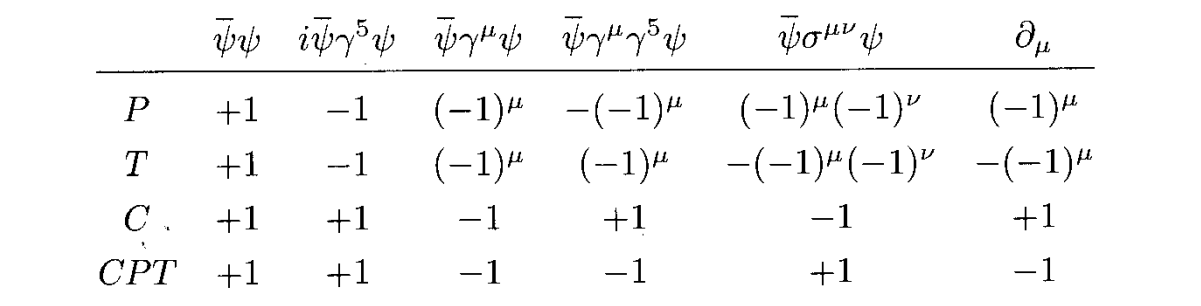
\includegraphics[height=3cm ,width=12cm]{QFT2/CPT.png}
\caption{Transformation of fermion bilinears under CPT}
\end{figure}

\begin{newthem}[CPT theorem]
Any hermitian combination of any set of fields (scalar, vector, Dirac, Majorana) and their derivatives that is a Lorentz scalar (and so carries no indices) is even under $CPT$. Since the Lagrangian must be formed out of such combinations, we
have $\mathcal{L}(x) \to \mathcal{L}(-x)$ under $CPT$, and so the action $S = \int d^4x \mathcal{L}$ is invariant.
\end{newthem}

\section{Perturbation theory for canonical quantization}
We use Yukawa theory as an example:
\[\mathcal{L} = -\frac{1}{2}\partial_{\mu} \phi \partial^{\mu} \phi -\frac{1}{2}M_0^2 \phi^2 + i\overline{\Psi} \gamma^{\mu} \partial_{\mu} \Psi - m_0\overline{\Psi}\Psi -g_0 \overline{\Psi}\Psi\phi.\]
\[H = H_0 + H_{\rm int} , \quad H_{\rm int} = \int d^3 x \: g_0 \overline{\Psi}\Psi\phi .\]
Similar to $\phi^4$ theory, the perturbation expansion of correlation functions is
\[\langle \Omega | T \{\Psi(x) \overline{\Psi}(y) \phi(z) \} | \Omega \rangle = \lim_{T \to \infty(1-i\epsilon)} \frac{\langle 0 | T \left\{ \Psi_{\rm I}(x) \overline{\Psi}_{\rm I}(y) \phi_{\rm I}(z) \mathrm{exp} \left[ -i \int_{-T}^{T} dt H_{\rm I} \right]\right\} | 0 \rangle}{\langle 0 | T \left\{ \mathrm{exp} \left[ -i \int_{-T}^{T} dt H_{\rm I} \right]\right\} | 0 \rangle}.\]
Before we state the Wick's theorem, we must note the following conventions:
\begin{enumerate}
\item  The time-ordered product picks up one minus sign for each interchange of operators that is necessary to put the fields in time order.
\item The normal-ordered product picks up one minus sign for each interchange of operators that is necessary to put the fields in normal order.
\item Define contractions under the normal-ordering symbol to include minus signs for operator interchanges.
\end{enumerate}
With these conventions, Wick's theorem takes the same form as before:
\[T \left\{ \Psi_{\rm I}(x_1) \overline{\Psi}_{\rm I}(x_2)  \Psi_{\rm I}(x_3) \cdots \right\} = N \left\{\Psi_{\rm I}(x_1) \overline{\Psi}_{\rm I}(x_2)  \Psi_{\rm I}(x_3) \cdots + \mbox{ all possible contractions }\right\} .\]
\begin{example}
\begin{eqnarray}
\langle 0 | T \left\{ \Psi_{{\rm I}a}(x_1) \overline{\Psi}_{{\rm I}b}(x_2) \Psi_{{\rm I}c}(x_3) \overline{\Psi}_{{\rm I}d}(x_4)\right\}| 0 \rangle &=& S_{\rm F}(x_1-x_2)_{ab}S_{\rm F}(x_3-x_4)_{cd} \nonumber \\
&-& S_{\rm F}(x_1-x_4)_{ad}S_{\rm F}(x_3-x_2)_{cb}. \nonumber
\end{eqnarray}
\end{example}

\noindent
Then we can derive the Feynman rule for Yukawa theory. 
Expand
\[\langle 0 | T \left\{ \Psi_{{\rm I}a}(x) \overline{\Psi}_{{\rm I}b}(y) \phi_{\rm I}(z) \mathrm{exp} \left[ -i \int_{-T}^{T} dt H_{\rm I} \right]\right\} | 0 \rangle\] 
to the first order of $g_0$
\begin{eqnarray}
& &\langle 0 | T \left\{ \Psi_{{\rm I}a}(x) \overline{\Psi}_{{\rm I}b}(y) \phi_{\rm {\rm I}}(z) (-i g_0) \int dw^4 \overline{\Psi}_{\rm I}(w) \Psi_{\rm I}(w) \phi_{\rm I}(w) \right\} | 0 \rangle \nonumber \\
&=& -(-ig_0) S_{\rm F}(x-y)_{ab} \int d^4 w D_{\rm F}(z-w) \mathrm{Tr}[S_{\rm F}(w-w)] \nonumber \\
&+&  (-ig_0) \int d^4 w  [S_{\rm F}(x-w) S_{\rm F}(w-y)]_{ab} D_{\rm F}(w-z) .\nonumber
\end{eqnarray}
It can be represented by the so called Feynman diagram.
\begin{figure}[!h]
\centering
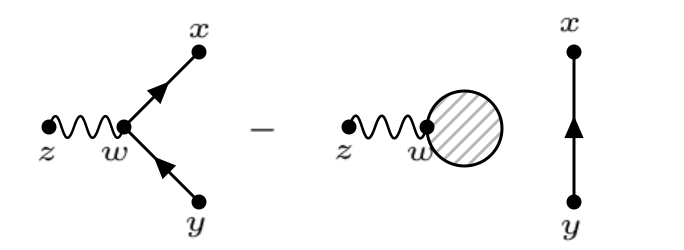
\includegraphics[height=2.6cm ,width=6.8cm]{QFT2/FD1.png}
\caption{Feynman diagram representation of perturbation expansion}
\end{figure}\\
The Feynman rules for Yukama theory are:
\begin{enumerate}
\item For each Fermion propagator from $y$ to $x$, $P = S_{\rm F}(x-y)$.
\item For each scalar propagator, $P = D_{\rm F}(x-y)$.
\item For each vertex, $V = (-ig_0)\int d^4w$.
\item For each external point, $E=1$.
\item Divided by the symmetry factor.
\end{enumerate}

\section{Path integral quantization}
\subsection{Grassmann numbers}
\subsubsection{Formal definition}
Grassmann numbers are individual elements or points of the exterior algebra generated by a set of $n$ Grassmann variables or Grassmann directions or supercharges $\{\theta _{i}\}$ with $n$ possibly being infinite.
The Grassmann variables are the basis vectors of a vector space (of dimension $n$). 
They form an algebra over a field, with the field usually being taken to be the complex numbers, although one could contemplate other fields, such as the reals. The algebra is a unital algebra, and the generators are anti-commuting:
\[\theta _{i}\theta _{j}=-\theta _{j}\theta _{i}.\]
Since the $\theta _{i}$ form a vector space over the complex numbers, it is trivial that they commute with the complex numbers; this is by definition. That is, for complex $x$, one has
\[\theta _{i}x=x\theta _{i}.\]
The squares of the generators vanish:
\[\theta_i \theta_i = -\theta_i \theta_i = 0.\]
In other words, a Grassmann variable is a non-zero square-root of zero.
Let $V$ denote this $n$-dimensional vector space of Grassmann variables. 
Note that it is independent of the choice of basis. The corresponding exterior algebra is defined as
\[\Lambda =\mathbb {C} \oplus V\oplus \left(V\wedge V\right)\oplus \left(V\wedge V\wedge V\right)\oplus \cdots\]
where $\wedge$ is the exterior product and $\oplus$ is the direct sum. The individual elements of this algebra are then called Grassmann numbers. It is standard to completely omit the wedge symbol $\wedge$ when writing a Grassmann number; it is used here only to clearly illustrate how the exterior algebra is built up out of the Grassmann variables. Thus, a completely general Grassmann number can be written as
\[z=\sum _{k=0}^{\infty }\sum _{i_{1},i_{2},\cdots ,i_{k}}c_{i_{1}i_{2}\cdots i_{k}}\theta _{i_{1}}\theta _{i_{2}}\cdots \theta _{i_{k}},\]
where the $c$s are complex numbers, or, equivalently, $c_{i_{1}i_{2}\cdots i_{k}}$ is a complex-valued, completely antisymmetric tensor of rank $k$. Again, the $\theta _{i}$ can be clearly seen here to be playing the role of a basis vector of a vector space.
Observe that the Grassmann algebra generated by $n$ linearly independent Grassmann variables has dimension $2^n$; this follows from the binomial theorem applied to the above sum, and the fact that the $n+1$-fold product of variables must vanish, by the anti-commutation relations, above. In other words, for $n$ variables, the sum terminates
\[\Lambda =\mathbb {C} \oplus \Lambda ^{1}V\oplus \Lambda ^{2}V\oplus \cdots \oplus \Lambda ^{n}V,\]
where $\Lambda ^{k}V$ is the k-fold alternating product. The dimension of  $\Lambda ^{k}V$ is given by $n$ choose $k$, the binomial coefficient. The special case of $n=1$ is called a dual number, and was introduced by William Clifford in 1873.

\subsubsection{Integral over Grassmann number}
\noindent
Single-variable:
\[\int d\theta (A + B\theta) \equiv B.\]
Multi-variable:
\[\int d\theta d\eta \; \eta \theta \equiv 1.\]
Complex Grassmann number:
\[(\theta \eta)^* \equiv \eta^* \theta^* = -\theta^* \eta^*.\]
\[\int d\theta^* d\theta \; \theta \theta^* \equiv 1.\]
Gaussian integral over a complex Grassmann number:
\[\int d\theta^* d\theta e^{-\theta^* b \theta} = b.\]
\[\int d\theta^* d\theta \; \theta \theta^* e^{-\theta^* b \theta}  = 1.\]
Unitary transformation:
If $\theta'_i = U_{ij}\theta_j$ and $U$ is unitary matrix, then we can derive
\[\prod_i \theta'_i = (\det U) (\prod_i \theta_i).\]
In a general integral
\[(\prod_i \int d\theta^*_i d\theta_i) f(\theta),\]
the only term of $f(\theta)$ that survives has exactly one factor of each $\theta_i$ and $\theta^*_i$; it is proportional to $(\prod_i \theta_i)(\prod_i \theta^*_i)$. If we replace $\theta$ by $U\theta$, this term acquires a factor of $\det U \det U^* = 1$, so the integral is unchanged under the unitary transformation.
Gaussian integral over multiple complex Grassmann numbers:
\[(\prod_i \int d\theta^*_i d\theta_i) e^{-\theta^*_i B_{ij}\theta_j} = \det B.\]
\[(\prod_i \int d\theta^*_i d\theta_i) \theta_k \theta^*_l e^{-\theta^*_i B_{ij}\theta_j} =B^{-1}_{kl} \det B.\]

\subsection{Path integral formulation for free Dirac field}
A Grassmann field is a function of space-time whose values are Grassmann numbers. The classical Dirac field being used to evaluate path integral is a Grassmann field. The correlation function is given by
\[\langle \Omega | T \Psi_{\rm H}(x_1) \overline{\Psi}_{\rm H}(x_2)| \Omega \rangle = \lim_{T \to \infty(1-i\epsilon)} \frac{\int \mathcal{D}\overline{\Psi} \mathcal{D}\Psi \; \mathrm{exp} \left[ i\int_{-T}^T d^4x \overline{\Psi}(i\slashed{\partial}-m)\Psi \right] \Psi(x_1) \overline{\Psi}(x_2)}{\int \mathcal{D}\overline{\Psi} \mathcal{D}\Psi \; \mathrm{exp} \left[ i\int_{-T}^T d^4x \overline{\Psi}(i\slashed{\partial}-m)\Psi \right]}.\]
The generating function is 
\[Z[\overline{\eta},\eta] = \int \mathcal{D}\overline{\Psi} \mathcal{D}\Psi \; \mathrm{exp} \left[ i\int d^4x \overline{\Psi}(i\slashed{\partial}-m)\Psi + \overline{\eta}\Psi + \overline{\Psi}\eta \right],\]
where $\eta(x)$ is a Grassmann-valued source field. 
Define
\[\Psi'(x) \equiv \Psi(x) - i \int d^4y S_{\rm F}(x-y)\eta(y).\]
Then we can derive that
\[\overline{\Psi}'(x) \equiv \overline{\Psi}(x) - i \int d^4y \overline{\eta}(y)S_{\rm F}(y-x).\]
Recall that
\[(i\slashed{\partial}_x-m)S_{\rm F}(x-y) = i\delta(x-y)\]
and
\[S_{\rm F}(y-x)(i \slashed{\partial}_x+m) = -i\delta(x-y).\]
We can derive that
\[\int d^4x \overline{\Psi}(i\slashed{\partial}-m)\Psi + \overline{\eta}\Psi + \overline{\Psi}\eta = \int d^4x \overline{\Psi}'(i\slashed{\partial}-m)\Psi' + i \int d^4x d^4y \overline{\eta}(x)S_{\rm F}(x-y)\eta(y) .\]
After integration, we have
\[Z[\overline{\eta},\eta] = Z[0] \mathrm{exp} \left[ -\int d^4x d^4y \; \overline{\eta}(x)S_{\rm F}(x-y)\eta(y) \right].\]
If we adopt the convention that
\[\frac{d}{d\eta} \theta \eta = - \frac{d}{d\eta} \eta \theta = - \theta,\]
the two point correlation functions are
\[\langle 0 | T \Psi_{\rm H}(x_1) \overline{\Psi}_{\rm H}(x_2)| 0 \rangle = Z[0]^{-1} \left(-i \frac{\delta}{\delta \overline{\eta}(x_1)} \right) \left(i \frac{\delta}{\delta \eta(x_2)} \right) Z[\overline{\eta},\eta]|_{\overline{\eta},\eta=0} = S_{\rm F}(x_1-x_2) .\]

\subsection{Perturbation theory for path integral quantization}
We use Yukawa theory as an example:
\begin{eqnarray}
\mathcal{L} &=& -\frac{1}{2}\partial_{\mu} \phi \partial^{\mu} \phi -\frac{1}{2}M_0^2 \phi^2 + i\overline{\Psi} \gamma^{\mu} \partial_{\mu} \Psi - m_0\overline{\Psi}\Psi -g_0 \overline{\Psi}\Psi\phi. \nonumber \\
\mathcal{L} &=& \mathcal{L}_0 + \mathcal{L}_1 , \quad \mathcal{L}_1 =- g_0\overline{\Psi}\Psi\phi .\nonumber \\
Z[J] &=& \int \mathcal{D}\phi \mathcal{D}\overline{\Psi} \mathcal{D}\Psi e^{i\int d^4x [\mathcal{L}_0 + \mathcal{L}_1 + J\phi + \overline{\eta}\Psi +  \overline{\Psi}\eta]} \nonumber \\
&=& e^{i\int d^4x \mathcal{L}_1(\frac{1}{i} \frac{\delta}{\delta J(x)},\frac{1}{i}\frac{\delta}{\delta \overline{\eta}(x)},-\frac{1}{i}\frac{\delta}{\delta \eta(x)})} \int \mathcal{D}\phi \mathcal{D}\overline{\Psi} \mathcal{D}\Psi e^{i\int d^4y [\mathcal{L}_0 + J\phi + \overline{\eta}\Psi +  \overline{\Psi}\eta]} \nonumber \\
&\propto & e^{i\int d^4x \mathcal{L}_1(\frac{1}{i} \frac{\delta}{\delta J(x)},\frac{1}{i}\frac{\delta}{\delta \overline{\eta}(x)},-\frac{1}{i}\frac{\delta}{\delta \eta(x)})} \mathrm{exp} [- \int d^4y d^4z  \frac{1}{2} J(y)D_{\rm F}(y-z)J(z) + \overline{\eta}(y)S_{\rm F}(y-z)\eta(z)] \nonumber \\
& =& \sum_{V=0}^{\infty} \frac{1}{V!} [-ig_0 \int d^4x (\frac{1}{i} \frac{\delta}{\delta J(x)}  \cdot -\frac{1}{i}\frac{\delta}{\delta \eta(x)} \cdot \frac{1}{i}\frac{\delta}{\delta \overline{\eta}(x)})]^V \nonumber \\
&\times & \sum_{P_1=0}^{\infty} \frac{1}{P_1!} [-\frac{1}{2} \int d^4y_1 d^4z_1 J(y_1)D_{\rm F}(y_1-z_1)J(z_1)]^{P_1} \nonumber \\
&\times &  \sum_{P_2=0}^{\infty} \frac{1}{P_2!} [-\int d^4y_2 d^4z_2 \overline{\eta}(y_2)S_{\rm F}(y_2-z_2)\eta(z_2)]^{P_2} .\nonumber
\end{eqnarray}
If we focus on a term with particular values of $V$, $P_1$ and $P_2$, then the number of surviving scalar sources is $E_1 = 2P_1-V$, the number of surviving fermion sources is $E_2 = 2P_2-2V$.
We can introduce Feynman diagrams as in the $\phi^4$ theory. In these diagrams, a dashed line segment stands for a scalar propagator $D_{\rm F}(x-y)$, a line with an arrow pointing from $y$ to $x$ for a fermion propagator $S_{\rm F}(x-y)$, a filled circle at one end of a dashed line segment for a scalar source $i\int d^4x J(x)$, a filled circle at the start of a line with an arrow for a fermion source $i\int d^4x \eta(x)$, a filled circle at the end of a line with an arrow for a anti-fermion source $i\int d^4x \overline{\eta}(x)$, a vertex joining three line segments for $-ig_0\int d^4x$.

\section{LSZ reduction formula}
Similarly to the scalar field theory, we can derive the structure of the exact propagator of Dirac fermions in interaction theory.
\[\int d^4x \; e^{-ipx} \langle \Omega | T \Psi(x) \overline{\Psi}(0) | \Omega \rangle_C = \frac{iZ_2(\slashed{p}-m)}{p^2+m^2-i\epsilon} + \cdots \]
We eliminate the terms contributing none isolate poles for $p^2$. Here, $m$ is the exact mass of the fermions. The constant $Z_2$ is the probability for the quantum field to create or annihilate an exact one-particle eigenstate of $H$:
\[\langle \Omega | \Psi(0) | p,s \rangle = \sqrt{Z_2} u^s(p).\]
The LSZ reduction formula for fermions would take the form as following.
\\

\begin{newthem}[LSZ reduction formula]
\begin{eqnarray}
&\phantom{=}& \langle \bm{p}_1 \cdots \bm{p}_n \;
\overline{\bm{p}}_1 \cdots \overline{\bm{p}}_{\overline{n}} \;
| S | \;
\bm{k}_1 \cdots \bm{k}_m \;
\overline{\bm{k}}_1 \cdots \overline{\bm{k}}_{\overline{n}} \rangle 
\nonumber \\
&=& , \quad \prod_1^n \int d^4 x_i e^{-i p_ix_i }
\prod_1^{\overline{n}} \int d^4 \overline{x}_i e^{-i \overline{p}_i\overline{x}_i }
\prod_1^m \int d^4 y_j e^{ik_jy_j}
\prod_1^{\overline{m}} d^4 \overline{y}_i e^{i\overline{k}_j\overline{y}_j}
\nonumber \\
&\times & [\overline{u}_{s_1}(\bm{p}_1)(\slashed{p}_1+m)] \cdots [\overline{u}_{s_n}(\bm{p}_n)(\slashed{p}_n+m)]
\nonumber \\
&\times & [\overline{v}_{\overline{r}_1}(\overline{\bm{k}}_1)(\overline{\slashed{k}}_1 - m)] \cdots [\overline{v}_{\overline{r}_{\overline{m}}}(\overline{\bm{k}}_{\overline{m}})(\overline{\slashed{k}}_{\overline{m}} - m)]
\nonumber \\
&\times & \langle \Omega | T \{\Psi(x_1) \cdots \Psi(x_n)
\overline{\Psi}(\overline{x}_1) \cdots \overline{\Psi}(\overline{x}_{\overline{n}}) 
\overline{\Psi}(y_1) \cdots \overline{\Psi}(y_m)
\Psi(\overline{y}_1) \cdots \Psi(\overline{y}_{\overline{m}})\} 
| \Omega \rangle 
\nonumber \\
&\times & [(\slashed{k}_1+m) u_{r_1}(\bm{k}_1)] \cdots [(\slashed{k}_m+m)u_{r_m}(\bm{k}_m)] \nonumber \\
&\times & [(\overline{\slashed{p}}_1 - m) v_{\overline{s}_1}(\overline{\bm{p}}_1)] \cdots [(\overline{\slashed{p}}_{\overline{n}} - m) v_{\overline{s}_{\overline{n}}}(\overline{\bm{p}}_{\overline{n}})] \nonumber \\
&\times & \left( \frac{i}{\sqrt{Z}_2} \right) ^{m+\overline{m}+n+\overline{n}} .\nonumber
\end{eqnarray}
\end{newthem}

\noindent
From this equation, we can see that the scattering amplitude would vanish unless $n+\overline{m} = \overline{n} + m$, which implies the conservation of $Q$. The term $e^{ipx}$ will impose the condition of momentum conservation, and the the term $\slashed{p}\pm m$ will remove the external legs.
Finally, we list the Feynman rules of Yukawa theory in momentum space as follows:
\begin{enumerate}
\item For each incoming electron, draw a solid line with an arrow pointed towards the vertex, and label it with the electron's four-momentum, $k_i$.
\item For each outgoing electron, draw a solid line with an arrow pointed away from the vertex, and label it with the electron's four-momentum, $p_i$.
\item For each incoming positron, draw a solid line with an arrow pointed away from the vertex, and label it with minus the positron's four-momentum, $-\bar{k}_i$.
\item For each outgoing positron, draw a solid line with an arrow pointed towards the vertex, and label it with minus the positron's four-momentum, $-\bar{p}_i$.
\item For each incoming scalar, draw a dashed line with an arrow pointed towards the vertex, and label it with the scalar's four-momentum, $q_i$.
\item For each outgoing scalar, draw a dashed line with an arrow pointed away from the vertex, and label it with the scalar's four-momentum, $q'_i$.
\item The only allowed vertex joins two solid lines, one with an arrow pointing towards it and one with an arrow pointing away from it, and one dashed line (whose arrow can point in either direction). Using this vertex, join up all the external lines, including extra internal lines as needed. In this way, draw all possible diagrams that are topologically inequivalent.
\item Assign each internal line its own four-momentum. Think of the four-momenta as flowing along the arrows, and conserve four-momentum at each vertex. For a tree diagram, this fixes the momenta on all the internal lines.
\item The value of a diagram consists of the following factors:
\begin{itemize}
\item for each incoming or outgoing scalar, $1$;
\item for each incoming electron, $u_{r}(\bm{k})$;
\item for each outgoing electron, $\overline{u}_{s}(\bm{p})$;
\item for each incoming positron, $\overline{v}_{\overline{r}}(\overline{\bm{k}})$;
\item for each outgoing positron, $v_{\overline{s}}(\overline{\bm{p}})$;
\item for each vertex, $-ig_0$;
\item for each internal scalar, ${-i}/{(p^2+M^2-i\epsilon)}$;
\item for each internal fermion, ${i(\slashed{p}-m)}/{(p^2+m^2-i\epsilon)}$.
\end{itemize}
\item Spinor indices are contracted by starting at one end of a fermion line: specifically, the end that has the arrow pointing away from the vertex. The factor associated with the external line is either $\bar{u}$ or $\bar{v}$. Go along the complete fermion line, following the arrows backwards, and write down (in order from left to right) the factors associated with the vertices and propagators that you encounter. The last factor is either a $u$ or $v$. Repeat this procedure for the other fermion lines, if any.
\item The overall sign of a tree diagram is determined by drawing all contributing diagrams in a standard form: all fermion lines horizontal, with their arrows pointing from left to right, and with the left endpoints labeled in the same fixed order (from top to bottom); if the ordering of the labels on the right endpoints of the fermion lines in a given diagram is an even (odd) permutation of an arbitrarily chosen fixed ordering, then the sign of that diagram is positive (negative).
\item Each closed fermion loop contributes an extra minus sign.
\item Value of $i\mathcal{M}$ is given by a sum over the values of the contributing diagrams.
\item $\langle f | S | i \rangle = (Z_1)^{\frac{n_s}{2}} (Z_2)^{\frac{n_f}{2}}i\mathcal{M}\delta(\sum p_f -\sum p_i)$.
\end{enumerate}

\section{Functional determinant}
We consider a theory of a Dirac fermion $\Psi$ with
\[\mathcal{L} = i\overline{\Psi} \gamma^{\mu} \partial_{\mu} \Psi - m\overline{\Psi}\Psi -g \overline{\Psi}\Psi\phi,\]
where $\phi$ is again a real scalar background field. We define the path integral
\[Z(\phi) = \int \mathcal{D}\overline{\Psi}\mathcal{D}\Psi e^{i\int d^4x \mathcal{L}} .\]
Recall that if we have $N$ complex Grassmann variables $\theta_i$, then we can evaluate gaussian integrals by the general formula
\[\int d^n\theta^* d\theta \exp[-i\theta^{*}_i M_{ij}\theta_j] \propto \det M.\]
In the case of the functional integral,the matrix $M$ becomes
\[M_{\alpha\beta}(x,y) = (-i\slashed{\partial}_x + m + g\phi(x))_{\alpha\beta}\delta(x-y).\]
We define
\[M_{0\alpha\beta}(x,y) \equiv (-i\slashed{\partial}_x + m )_{\alpha\beta}\delta(x-y),\]
\[M_{1\beta\gamma}(y,z) \equiv \delta_{\beta\gamma}\delta(y-z) + igS_{\rm F}(y-z)_{\beta\gamma}\phi(z).\]
We can verify that
\[M_{\alpha\gamma}(x,z) = \int d^4y M_{0\alpha\beta}(x,y)M_{1\beta\gamma}(y,z) .\]
Furthermore, we have $M_1 = I - G$, where $I$ is the identity matrix and
\[G_{\alpha\beta}(x-y) = -igS_{\rm F}(x-y)_{\alpha\beta}\phi(x).\]
Thus
\[\log Z[\phi] = \log \det M_1 = -\sum_{n=1}^{\infty} \frac{1}{n} \mathrm{Tr}G^n,\]
where now
\[\mathrm{Tr}G^n = (-ig)^n \int d^4x_1 \cdots d^4x_n \mathrm{tr} S_{\rm F}(x_1-x_2)\phi(x_2) \cdots S_{\rm F}(x_n-x_1)\phi(x_1)\]
and ``tr'' denotes a trace over spinor indices.
\\ \\
To better understand what it means, we will rederive it in a different way. 
Consider treating the $-g\phi\overline{\Psi}\Psi$ term in $\mathcal{L}$ as an interaction. This leads to a vertex that connects two $\Psi$ propagators; the associated vertex factor
is $-ig\phi(x)$. 
Thus we have
\[\log Z[\phi] = \sum_{I}C_I,\]
where $C_I$ represents connected diagram without external source. The only connected diagrams we can draw with these Feynman rules are fermion circles with $n$ vertices. 
The has an $n$-fold cyclic symmetry, leading to a symmetry factor of $S= n$. The closed fermion loop implies a trace over the spinor indices. Thus the value of the $n$-vertex diagram is
\[\frac{1}{n}(-ig)^n \int d^4x_1 \cdots d^4x_n \mathrm{tr} S_{\rm F}(x_1-x_2)\phi(x_2) \cdots S_{\rm F}(x_n-x_1)\phi(x_1).\]
Summing up these diagrams, we find that we are missing the overall minus sign. The appropriate conclusion is that we must associate an extra minus sign with each closed fermion loop.